% options:
% thesis=B bachelor's thesis
% thesis=M master's thesis
% czech thesis in Czech language
% slovak thesis in Slovak language
% english thesis in English language
% hidelinks remove colour boxes around hyperlinks

\documentclass[thesis=M,czech]{FITthesis}[2012/06/26]

\usepackage[utf8]{inputenc} % LaTeX source encoded as UTF-8

\usepackage{graphicx} %graphics files inclusion
% \usepackage{amsmath} %advanced maths
% \usepackage{amssymb} %additional math symbols

\usepackage{dirtree} %directory tree visualisation

% % list of acronyms
% \usepackage[acronym,nonumberlist,toc,numberedsection=autolabel]{glossaries}
% \iflanguage{czech}{\renewcommand*{\acronymname}{Seznam pou{\v z}it{\' y}ch zkratek}}{}
% \makeglossaries

\newcommand{\tg}{\mathop{\mathrm{tg}}} %cesky tangens
\newcommand{\cotg}{\mathop{\mathrm{cotg}}} %cesky cotangens

% % % % % % % % % % % % % % % % % % % % % % % % % % % % % % 
% ODTUD DAL VSE ZMENTE
% % % % % % % % % % % % % % % % % % % % % % % % % % % % % % 

\department{Katedra softwarového inženýrství}
\title{Letecké záznamy pro iOS pomocí moderních architektur a FRP}
\authorGN{Martin} %(křestní) jméno (jména) autora
\authorFN{Žid} %příjmení autora
\authorWithDegrees{Bc. Martin Žid} %jméno autora včetně současných akademických titulů
\author{Martin Žid} %jméno autora bez akademických titulů
\supervisor{Ing. Dominik Veselý}

\acknowledgements{Doplňte, máte-li komu a za co děkovat. V~opačném případě úplně odstraňte tento příkaz.}

\abstractCS{
%TOTO NENI FINALNI VERZE
Tato práce realizuje iOS aplikaci pro evidenci letů.  Práce analyzuje obdobné aplikace a předpisy pro piloty České republiky, podle nichž probíhá návrh funkcionality vytvářené aplikace. Podle návrhu je následně zvolena vhodná architektura a vytvořeno uživatelského rozhraní v podobě wireframů.

Aplikace je implementována s použitím zvolené architektury a pomocí principů FRP. V průběhu implementace aplikace jsou realizovány jednotkové testy a na konci jsou provedeny uživatelské testy. Na základě výsledků testů je aplikace upravena do finální podoby.

V~práci jsem vytvořil funkční iOS aplikaci s využitím moderní architektury a principů FRP. Aplikace bude sloužit pilotům České republiky pro elektronickou evidenci letů a bude jim také ulehčovat administrativu s evidencí spojenou.

V~příloze této bakalářské práce je možné nalézt
všechny zdrojové kódy jak aplikace, tak i testů společně s~vytvořenými wireframy.
}

\abstractEN{Sem doplňte ekvivalent abstraktu Vaší práce v~angličtině.}

\placeForDeclarationOfAuthenticity{V~Praze}
\declarationOfAuthenticityOption{4} %volba Prohlášení (číslo 1-6)
\keywordsCS{mobilní aplikace pro evidenci letů, iOS, Swift, FRP, ReactiveCocoa, MVVM architektura}
\keywordsEN{flight records mobile application, iOS, Swift, FRP, ReactiveCocoa, MVVM architecture}

\begin{document}

% \newacronym{CVUT}{{\v C}VUT}{{\v C}esk{\' e} vysok{\' e} u{\v c}en{\' i} technick{\' e} v Praze}
% \newacronym{FIT}{FIT}{Fakulta informa{\v c}n{\' i}ch technologi{\' i}}

\begin{introduction}
V dnešní době, kdy existují mobilní aplikace na téměř vše, mě zarazil fakt, že u pilotů tomu tak nemusí být. Aplikace na evidenci letů samozřejmě existují, však je tu hned několik problémů. Ty aplikace jsou často velice drahé, nemusí odpovídat leteckým přepisům České republiky nebo nemají vyhovující funkcionalitu.

Z tohoto důvodu jsem se rozhodl vytvořit iOS aplikaci na evidenci letů. Tato aplikace bude pomáhat pilotům zaznamenávat elektronicky své lety, bude také kontrolovat předpisy a umožňovat export do formátu pro tisk.

Začínám analýzou podobných aplikací a to pro zařízení iOS i Android. Poté navrhuji vhodnou funkcionalitu a vytvářím návrh uživatelského rozhraní.

Dalším tématem, které ve své práci řeším jsou softwarové architektury při vývoji iOS aplikace. Zde analyzuji alternativy k architektuře MVC ve spojení s funkcionálně reaktivním programováním neboli FRP.

Tuto analýzu následně aplikuji v praxi, kdy se zvolenou architekturou a FRP implementuji společně s jednotkovými testy dříve zmíněnou aplikaci. Nakonec aplikaci podrobím uživatelským testům a podle jejich výsledků
upravím aplikaci do finální podoby.

V poslední části své práce se snažím zhodnotit postupy FRP společně s mnou zvolenou moderní architekturou a jejich časovou a implementační náročnost oproti klasickému MVC.
\end{introduction}

\chapter{Cíl práce}

\chapter{Analýza a návrh}
\section{Architektury při tvorbě iOS aplikací}
Při tvorbě iOS aplikace je možné si vybrat z několika architektur. V této kapitole budu rozebírat pouze MVC, MVVM a VIPER.

\subsection{MVC}
Architektura MVC je zkratka pro \uv{Model View Controller} neboli tři komponenty, ze kterých se architektura skládá. Jedná se o softwarovou architekturu, které se velice často používá při tvorbě aplikací s uživatelským rozhraním. \cite{MVCMozilla}
\begin{itemize}
\item $Model$ definuje jaká data aplikace obsahuje a pokud dojde k jakékoliv změně, tak informuje buď $Controller$ nebo $View$ (tzv. své observery). \cite{MVCGoogle}
\item $View$ vrstva je prezentována samotnému uživateli. Tedy jsou zde zobrazena aplikační data a je zachycována uživatelova práce s aplikací.\cite{MVCMozilla}
\item $Controller$ je vrstva mezi $View$ a $Model$ zabezpečující logiku aplikace. Stará se o promítnutí změn do $View$ pokud se změní $Model$. Zároveň provádí úpravy v $Model$ při uživatelově manipulaci s $View$.  \cite{MVCGoogle}
\end{itemize}

Však co se týče iOS vývoje, vrstvy $View$ a $Controller$ jsou téměř spojeny, protože $Controller$ je příliš úzce zapojený do životního cyklu $View$. Což následně způsobuje velký nárůst $Controller$.\cite{Orlov}

Základní myšlenku MVC a MVC při vývoji iOS aplikace ukazují obrázky \ref{fig:mvc} a \ref{fig:mvc-apple}.

MVC je základní architekturou pro tvorbu iOS aplikací. Není však jedinou možností.

\begin{figure}[h]\centering
 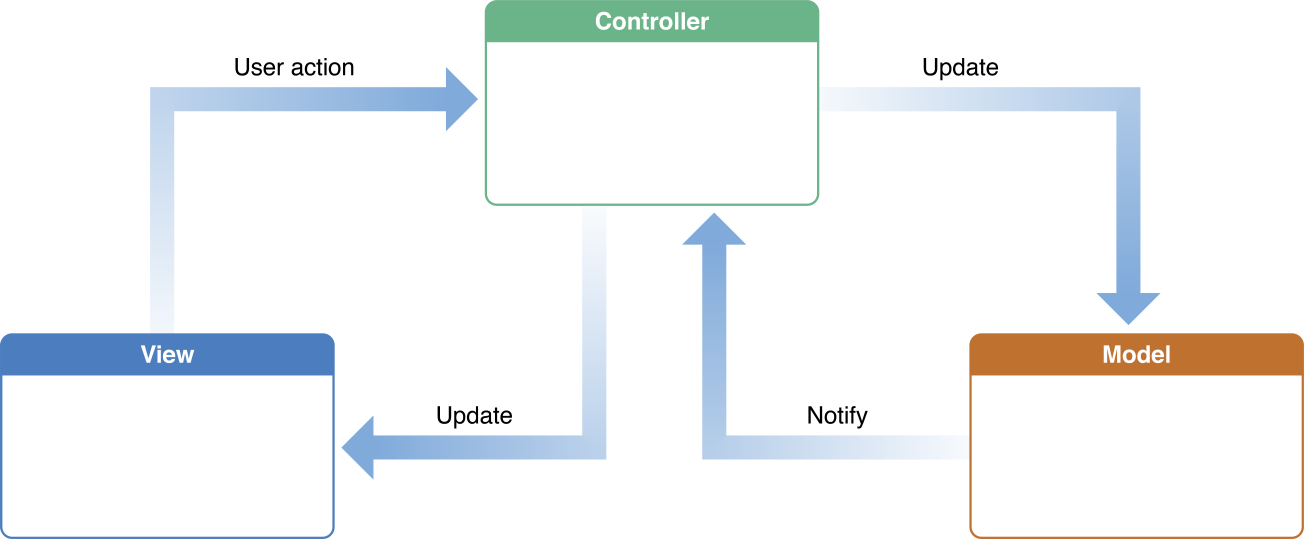
\includegraphics[width=0.99\textwidth]{./pictures/architektury/model_view_controller}
 \caption[Model-View-Controller diagram]{Model-View-Controller diagram \cite{mvc-pic}}\label{fig:mvc}
\end{figure}

\begin{figure}[h]\centering
 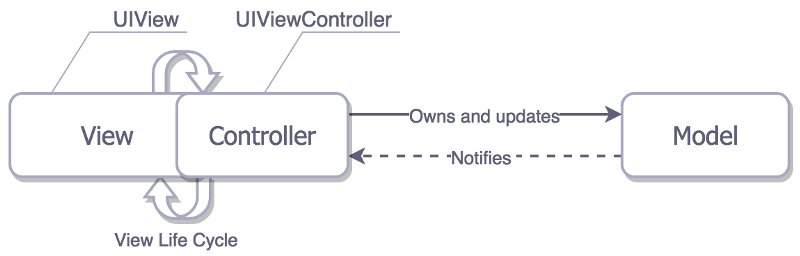
\includegraphics[width=0.99\textwidth]{./pictures/architektury/appleMVC}
 \caption[Model-View-Controller při vývoji iOS aplikace]{Model-View-Controller při vývoji iOS aplikace \cite{mvc-apple-pic}}\label{fig:mvc-apple}
\end{figure}

\subsection{MVVM}
Architektura MVVM má obdobné koncepce jako MVC. Jedná se také o zkratku, tentokrát \uv{Model-View-ViewModel}. \cite{MVVMMicrosoft}
\begin{itemize}
\item $Model$ je totožný s $Model$ vrstvou architektury MVC, jedná se tedy o datovou část aplikace.
\item $View$ prezentuje aplikační data uživateli a monitoruje jeho akce. Však, jak již bylo zmíněno dříve, u iOS aplikací se jedná spíše o vrstvu\\ $View/View controller$. Tato vrstva obsahuje pouze minimum logiky aplikace a reaguje hlavně na $ViewModel$.  \cite{Morrison}
\item $ViewModel$ spojuje $View$ a $Model$ a zajišťuje hlavní logiku aplikace. $ViewModel$ tedy komunikuje s  $Model$ a jeho metodami a následně připravuje data pro $View$. Obsahuje také implementaci funkcí, které reagují a zpracovávají akce uživatele, např.: kliknutí na tlačítko. \cite{MVVMMicrosoft}
\end{itemize}

Tedy pro shrnutí rozdílů MVC a MVVM u iOS bych zmínil to, že iOS MVC má ve výsledku téměř jen dvě vrstvy $View/View controller$ a $Model$. Když potom uvažujeme architekturu MVVM $View/View controller$  je opravdu pouze jednou vrstvou a mezi ní a $Model$ je vložena nová vrstva  $ViewModel$, která je spojuje a do které je přesunuta i většina aplikační logiky.

Mezi výhody architektury MVVM oproti MVC patří např.:
\begin{itemize}
\item poskytuje návrhový princip tzv. separation of concerns, neboli oddělení zájmů;
\item zlepšuje možnost testovatelnosti aplikace.
\end{itemize}

\begin{figure}[h]\centering
 \includegraphics[width=0.99\textwidth]{./pictures/architektury/MVVM}
 \caption[Model-View-ViewModel architektura]{Model-View-ViewModel architektura \cite{mvvm-pic}}\label{fig:mvvm}
\end{figure}

\subsection{VIPER}
VIPER je poslední rozebíranou možností, co se týče architektur. I zde je název složen z prvních písmen jednotlivých vrstev architektury, tedy \uv{View, Interactor, Presenter, Entity, Router}.
\begin{itemize}
\item $View$  zobrazuje data uživateli a předává uživatelovi vstupy vrstvě $Presenter$.
\item $Interactor$ obsahuje logiku aplikace spojenou s daty ($Entity$).
\item $Presenter$ vrstva má na starosti $View$ logiku.  Reaguje tedy na uživatelovi akce a komunikuje s vrstvou $Interactor$, od ní také přijímá nová data. \cite{Orlov}
\item $Entity$ jsou datové objekty aplikace přístupné pouze části $Interactor$.
\item $Routing$ obsahuje navigační logiku. \cite{VIPER}
\end{itemize}

Mezi výhody architektury VIPER znovu patří např.:
\begin{itemize}
\item dobře rozděluje odpovědnosti;
\item zlepšuje možnost testovatelnosti aplikace. \cite{Orlov}
\end{itemize}

Tato architektura však může být příliš náročná a přehnaná pro menší aplikace. \cite{Orlov}

\begin{figure}[h]\centering
 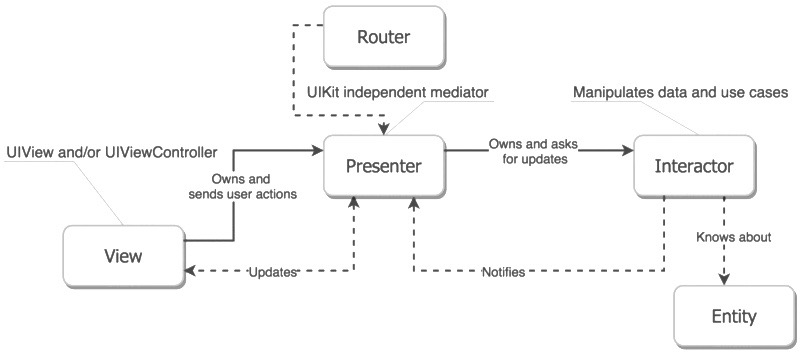
\includegraphics[width=0.99\textwidth]{./pictures/architektury/viper.jpg}
 \caption[VIPER architektura]{VIPER architektura \cite{viper-pic}}\label{fig:viper}
\end{figure}

\section{Funkcionálně reaktivní programování}
Podle \cite{technopediaFRP} je funkcionálně reaktivní programování kombinací funkcionálního a reaktivního programování. Díky němuž dokáže aplikace dynamicky měnit stav a chování v závislosti na událostech přicházejících za nějaký čas.

Pro vysvětlení, co je reaktivní programování cituji \cite{Ztaltz2014} \uv{reaktivní programování je programování s asynchronními datovými toky}.

Na spojení funkcionální a reaktivního programování může dívat i jako na návrhový vzor $observer$. \cite{Blackheath2016} Pozorujeme tedy např. určité vstupní pole, tlačítko, nebo i dotaz na server a jsme informování o každé změně v podobě asynchronního datového toku. Na tyto datové toky je možné aplikovat funkcionální programování. Je tedy možné toky spojovat ($merge$), filtrovat ($filter$) pouze události, které nás zajímají,  mapovat ($map$) jeden tok na nový a další. \cite{Ztaltz2014}

\subsection{FRP frameworky pro iOS}
V této kapitole jsou pouze rozebrány základy jednotlivých frameworků, podrobnější vysvětlení společně s ukázkami jsou v k nalezení v kapitole Realizace.
\subsubsection{ReactiveSwift}
ReactiveSwift je prvním frameworkem pro iOS podporující FRP. Obsahuje řadu základních prvků ($Signal$, $SignalProducer$, $Property$, $Action$, \ldots) a operátorů podporujících myšlenku \uv{tok hodnot za čas}. \cite{ReactiveSwift}
\subsubsection{ReactiveCocoa}
ReactiveCocoa je další z FRP frameworků pro iOS. ReactiveCocoa rozšiřuje různé aspekty Apple Cocoa frameworku základními prvky frameworku ReactiveSwift. Umožňuje vazbu na prvky uživatelského rozhraní, u interaktivních prvků napojuje $Signal$ a $Action$ pro kontrolu událostí a změn. Dále také umožňuje vytvářet signály na volání metod (např. i pro UIKit třídy). \cite{ReactiveCocoa}


\chapter{Realizace}

\begin{conclusion}
	%sem napište závěr Vaší práce
\end{conclusion}

\bibliographystyle{csn690}
\bibliography{mybibliographyfile}

\appendix

\chapter{Seznam použitých zkratek}
% \printglossaries
\begin{description}
	\item[GUI] Graphical user interface
	\item[XML] Extensible markup language
\end{description}


% % % % % % % % % % % % % % % % % % % % % % % % % % % % 
% % Tuto kapitolu z výsledné práce ODSTRAŇTE.
% % % % % % % % % % % % % % % % % % % % % % % % % % % % 
% 
% \chapter{Návod k~použití této šablony}
% 
% Tento dokument slouží jako základ pro napsání závěrečné práce na Fakultě informačních technologií ČVUT v~Praze.
% 
% \section{Výběr základu}
% 
% Vyberte si šablonu podle druhu práce (bakalářská, diplomová), jazyka (čeština, angličtina) a kódování (ASCII, \mbox{UTF-8}, \mbox{ISO-8859-2} neboli latin2 a nebo \mbox{Windows-1250}). 
% 
% V~české variantě naleznete šablony v~souborech pojmenovaných ve formátu práce\_kódování.tex. Typ může být:
% \begin{description}
% 	\item[BP] bakalářská práce,
% 	\item[DP] diplomová (magisterská) práce.
% \end{description}
% Kódování, ve kterém chcete psát, může být:
% \begin{description}
% 	\item[UTF-8] kódování Unicode,
% 	\item[ISO-8859-2] latin2,
% 	\item[Windows-1250] znaková sada 1250 Windows.
% \end{description}
% V~případě nejistoty ohledně kódování doporučujeme následující postup:
% \begin{enumerate}
% 	\item Otevřete šablony pro kódování UTF-8 v~editoru prostého textu, který chcete pro psaní práce použít -- pokud můžete texty s~diakritikou normálně přečíst, použijte tuto šablonu.
% 	\item V~opačném případě postupujte dále podle toho, jaký operační systém používáte:
% 	\begin{itemize}
% 		\item v~případě Windows použijte šablonu pro kódování \mbox{Windows-1250},
% 		\item jinak zkuste použít šablonu pro kódování \mbox{ISO-8859-2}.
% 	\end{itemize}
% \end{enumerate}
% 
% 
% V~anglické variantě jsou šablony pojmenované podle typu práce, možnosti jsou:
% \begin{description}
% 	\item[bachelors] bakalářská práce,
% 	\item[masters] diplomová (magisterská) práce.
% \end{description}
% 
% \section{Použití šablony}
% 
% Šablona je určena pro zpracování systémem \LaTeXe{}. Text je možné psát v~textovém editoru jako prostý text, lze však také využít specializovaný editor pro \LaTeX{}, např. Kile.
% 
% Pro získání tisknutelného výstupu z~takto vytvořeného souboru použijte příkaz \verb|pdflatex|, kterému předáte cestu k~souboru jako parametr. Vhodný editor pro \LaTeX{} toto udělá za Vás. \verb|pdfcslatex| ani \verb|cslatex| \emph{nebudou} s~těmito šablonami fungovat.
% 
% Více informací o~použití systému \LaTeX{} najdete např. v~\cite{wikilatex}.
% 
% \subsection{Typografie}
% 
% Při psaní dodržujte typografické konvence zvoleného jazyka. České \uv{uvozovky} zapisujte použitím příkazu \verb|\uv|, kterému v~parametru předáte text, jenž má být v~uvozovkách. Anglické otevírací uvozovky se v~\LaTeX{}u zadávají jako dva zpětné apostrofy, uzavírací uvozovky jako dva apostrofy. Často chybně uváděný symbol "{} (palce) nemá s~uvozovkami nic společného.
% 
% Dále je třeba zabránit zalomení řádky mezi některými slovy, v~češtině např. za jednopísmennými předložkami a spojkami (vyjma \uv{a}). To docílíte vložením pružné nezalomitelné mezery -- znakem \texttt{\textasciitilde}. V~tomto případě to není třeba dělat ručně, lze použít program \verb|vlna|.
% 
%Více o~typografii viz \cite{kobltypo}.
% 
% \subsection{Obrázky}
% 
% Pro umožnění vkládání obrázků je vhodné použít balíček \verb|graphicx|, samotné vložení se provede příkazem \verb|\includegraphics|. Takto je možné vkládat obrázky ve formátu PDF, PNG a JPEG jestliže používáte pdf\LaTeX{} nebo ve formátu EPS jestliže používáte \LaTeX{}. Doporučujeme preferovat vektorové obrázky před rastrovými (vyjma fotografií).
% 
% \subsubsection{Získání vhodného formátu}
% 
% Pro získání vektorových formátů PDF nebo EPS z~jiných lze použít některý z~vektorových grafických editorů. Pro převod rastrového obrázku na vektorový lze použít rasterizaci, kterou mnohé editory zvládají (např. Inkscape). Pro konverze lze použít též nástroje pro dávkové zpracování běžně dodávané s~\LaTeX{}em, např. \verb|epstopdf|.
% 
% \subsubsection{Plovoucí prostředí}
% 
% Příkazem \verb|\includegraphics| lze obrázky vkládat přímo, doporučujeme však použít plovoucí prostředí, konkrétně \verb|figure|. Například obrázek \ref{fig:float} byl vložen tímto způsobem. Vůbec přitom nevadí, když je obrázek umístěn jinde, než bylo původně zamýšleno -- je tomu tak hlavně kvůli dodržení typografických konvencí. Namísto vynucování konkrétní pozice obrázku doporučujeme používat odkazování z~textu (dvojice příkazů \verb|\label| a \verb|\ref|).
% 
% \begin{figure}\centering
% 	
\includegraphics[width=0.5\textwidth, angle=30]{cvut-logo-bw}
% 	\caption[Příklad obrázku]{Ukázkový obrázek v~plovoucím prostředí}\label{fig:float}
% \end{figure}
% 
% \subsubsection{Verze obrázků}
% 
% % Gnuplot BW i barevně
% Může se hodit mít více verzí stejného obrázku, např. pro barevný či černobílý tisk a nebo pro prezentaci. S~pomocí některých nástrojů na generování grafiky je to snadné.
% 
% Máte-li například graf vytvořený v programu Gnuplot, můžete jeho černobílou variantu (viz obr. \ref{fig:gnuplot-bw}) vytvořit parametrem \verb|monochrome dashed| příkazu \verb|set term|. Barevnou variantu (viz obr. \ref{fig:gnuplot-col}) vhodnou na prezentace lze vytvořit parametrem \verb|colour solid|.
% 
% \begin{figure}\centering
% 	\includegraphics{gnuplot-bw}
% 	\caption{Černobílá varianta obrázku generovaného programem Gnuplot}\label{fig:gnuplot-bw}
% \end{figure}
% 
% \begin{figure}\centering
% 	\includegraphics{gnuplot-col}
% 	\caption{Barevná varianta obrázku generovaného programem Gnuplot}\label{fig:gnuplot-col}
% \end{figure}
% 
% 
% \subsection{Tabulky}
% 
% Tabulky lze zadávat různě, např. v~prostředí \verb|tabular|, avšak pro jejich vkládání platí to samé, co pro obrázky -- použijte plovoucí prostředí, v~tomto případě \verb|table|. Například tabulka \ref{tab:matematika} byla vložena tímto způsobem.
% 
% \begin{table}\centering
% 	\caption[Příklad tabulky]{Zadávání matematiky}\label{tab:matematika}
% 	\begin{tabular}{|l|l|c|c|}\hline
% 		Typ		& Prostředí		& \LaTeX{}ovská zkratka	& \TeX{}ovská zkratka	\tabularnewline \hline \hline
% 		Text		& \verb|math|		& \verb|\(...\)|	& \verb|$...$|		\tabularnewline \hline
% 		Displayed	& \verb|displaymath|	& \verb|\[...\]|	& \verb|$$...$$|	\tabularnewline \hline
% 	\end{tabular}
% \end{table}
% 
% % % % % % % % % % % % % % % % % % % % % % % % % % % % 

\chapter{Obsah přiloženého CD}

%upravte podle skutecnosti

\begin{figure}
	\dirtree{%
		.1 readme.txt\DTcomment{stručný popis obsahu CD}.
		.1 exe\DTcomment{adresář se spustitelnou formou implementace}.
		.1 src.
		.2 impl\DTcomment{zdrojové kódy implementace}.
		.2 thesis\DTcomment{zdrojová forma práce ve formátu \LaTeX{}}.
		.1 text\DTcomment{text práce}.
		.2 thesis.pdf\DTcomment{text práce ve formátu PDF}.
		.2 thesis.ps\DTcomment{text práce ve formátu PS}.
	}
\end{figure}

\end{document}
